\section{Fazit}

\subsection{Blockdiagramm der Gesamtlösung}
Die folgende Darstellung zeigt die Gesamtarchitektur der entwickelten Lösung. Sie umfasst die Kommunikation zwischen der KaVo Dentaleinheit (mit eingebetteter CONNECTbase-Software), dem lokalen Netzwerk, Home Assistant sowie der Stromsteuerung über Shelly Smart-Schalter.
\vspace{1cm}
\begin{figure}[H]
    \centering
    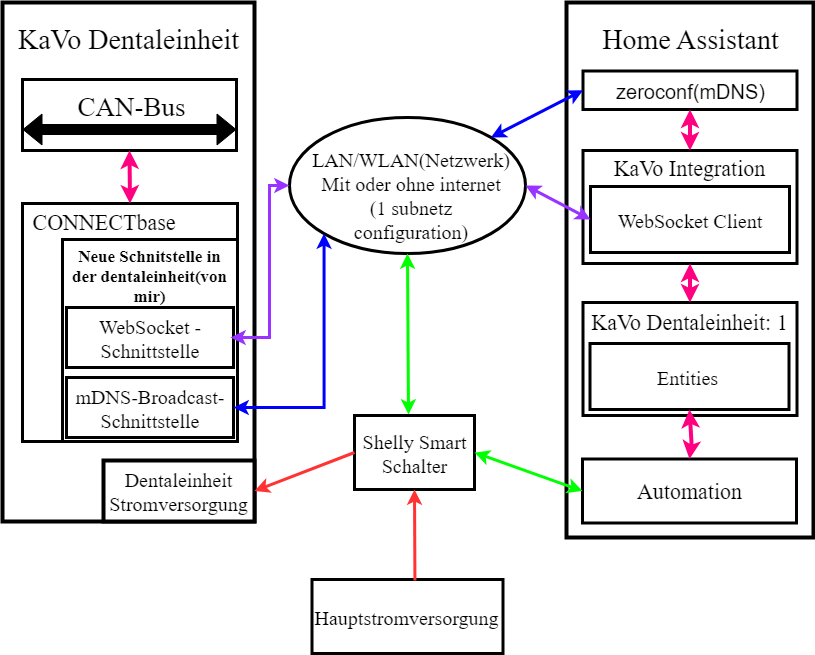
\includegraphics[width=\linewidth]{images/gesamtdiagram.drawio.png}
    \caption{Blockdiagramm der Gesamtlösung zur Integration mehrerer KaVo-Dentaleinheiten in Home Assistant}
    \label{fig:gesamtdiagramm}
\end{figure}

\textbf{Legende:}
\begin{itemize}
    \item \textcolor{blue}{\textbf{Blau:} mDNS-Kommunikation (Discovery über das Netzwerk)}
    \item \textcolor{magenta}{\textbf{Magenta:} WebSocket-Kommunikation (zwischen Home Assistant und Dentaleinheit)}
    \item \textcolor{green}{\textbf{Grün:} Steuerbefehle (z.\,B. smart schalter steuerung durch Automationen)}
    \item \textcolor{red}{\textbf{Rot:} Stromversorgung}
    \item \textcolor{strongpink}{\textbf{Pink:} Interne Kommunikation (z.\,B. CAN-Bus oder innerhalb von Home Assistant)}
\end{itemize}

\subsection{Voraussetzungen für einen zuverlässigen Betrieb mit 100 Geräten}

Um eine reibungslose und skalierbare Integration von bis zu 100 KaVo-Dentaleinheiten in einer lokalen Netzwerkumgebung sicherzustellen, sind bestimmte technische Rahmenbedingungen unerlässlich:

\begin{itemize}
    \item \textbf{Alle Geräte im selben Subnetz:} (z.\,B. 192.168.1.x)\\
    Dies ist notwendig für die mDNS-basierte Geräteerkennung, stabile WebSocket-Kommunikation und zuverlässige Automatisierung über Home Assistant. mDNS funktioniert ausschließlich innerhalb eines Subnetzes.\\
    Ein typisches IPv4-Subnetz (\texttt{/24}) erlaubt bis zu \textbf{254 eindeutige IP-Adressen}, wodurch sich auch größere Installationen mit über 100 Geräten problemlos abbilden lassen.\\

    \item \textbf{Verkabelung über Ethernet und Switches:}\\
    Geräte sollten idealerweise per LAN-Kabel mit einem zentralen Switch verbunden werden, um Verbindungsabbrüche durch Funkstörungen zu vermeiden – besonders in einer medizinischen Umgebung mit vielen elektromagnetischen Einflüssen.\\

    \item \textbf{WLAN nur über strukturierte Access-Point- oder Mesh-Systeme:}\\
    Wenn WLAN erforderlich ist, sollte es professionell geplant sein. Systeme wie \textit{Ubiquiti UniFi}, \textit{AVM Fritz!Mesh} oder \textit{TP-Link Omada} ermöglichen stabile Netzabdeckung mit dedizierten Backhauls. Ein einzelner Consumer-Router reicht für große Praxen nicht aus.\\
    
    Alternativ kann auf jedem Stockwerk eine eigene Home Assistant-Instanz mit eigenem Netzwerksegment betrieben werden, um die Last zu verteilen.\\

    \item \textbf{Statische IP-Adressen oder DHCP-Reservierungen:}\\
    Jede Dentaleinheit sollte immer unter derselben IP-Adresse erreichbar sein, um Home Assistant die dauerhafte Zuordnung zu ermöglichen. Dies kann über DHCP-Reservierung im Router oder manuell über feste IP-Adressen erfolgen.
\end{itemize}

\vspace{1em}
\noindent
\textbf{Warum funktioniert Home Assistant auch mit 100+ Geräten zuverlässig?}
\begin{itemize}
    \item KaVo Integration nutzt eine \textbf{asynchrone Architektur}, bei der Hintergrundprozesse (z.\,B. WebSocket-Clients) unabhängig voneinander laufen.\\
    
    \item Jedes Gerät verfügt über eine eigene WebSocket-Verbindung, deren Daten effizient verarbeitet und in zugehörige Entitäten überführt werden.\\
    
    \item \textbf{Automationen} reagieren nur auf spezifische Zustandsänderungen und sind so konfiguriert, dass sie \textbf{parallel} ausgeführt werden können. Dadurch entstehen keine Verzögerungen oder Blockaden.\\
    
    \item Die Entitätenstruktur in Home Assistant ermöglicht eine gezielte und performante Ereignisverarbeitung – auch bei vielen gleichzeitig aktiven Geräten.
\end{itemize}

\subsection{Zusammenfassung der Ergebnisse}

Im Verlauf dieser Arbeit wurden drei zentrale Bausteine umgesetzt, die gemeinsam eine lokal funktionierende, erweiterbare und echtzeitfähige Lösung für die Integration von KaVo Dentaleinheiten schaffen:

\begin{enumerate}
    \item \textbf{Schnittstelle zur externen Datenübertragung:}\\  
    Über die entwickelte WebSocket- und mDNS-basierte Schnittstelle kann die Dentaleinheit lokal in Echtzeit mit externen Systemen kommunizieren – ohne Umweg über eine Cloud. Die Testumgebung simuliert dieses Verhalten bereits erfolgreich und dient als Vorlage für eine zukünftige Implementierung direkt in die CONNECTbase-Software.\\

    \item \textbf{Externe Automatisierungs- und Visualisierungsplattform:}\\  
    Die speziell entwickelte KaVo Integration für Home Assistant ermöglicht eine zentrale Visualisierung des Stuhlstatus, die Abbildung hygienerelevanter Zeitpläne sowie flexible Automationen. Dabei bleibt die Lösung vollständig lokal und datenschutzfreundlich – ideal für klinische Umgebungen.\\

    \item \textbf{Automatisierte Steuerung der Stromversorgung ohne Eingriff in die bestehende Hardware:}\\  
    Durch den Einsatz eines \texttt{Shelly Pro 1PM} konnte eine einfache, kosteneffiziente Möglichkeit geschaffen werden, die Stromversorgung der Dentaleinheit automatisiert zu steuern. Die Integration erfolgt ohne jegliche Veränderung an der internen Elektronik und kann direkt über Home Assistant angesteuert werden.\\
\end{enumerate}

Die Kombination dieser drei Komponenten bildet eine lokal betriebene Lösung, die sowohl funktionale als auch nicht-funktionale Anforderungen erfüllt. Sie zeichnet sich durch Echtzeitfähigkeit, Erweiterbarkeit, geringe Latenz und Kosten sowie durch ihre vollständige Unabhängigkeit von Cloud-Diensten aus.

Ziel ist es, die Erkenntnisse aus dieser Arbeit künftig in die produktive CONNECTbase-Software zu überführen und damit die Basis für eine neue Generation vernetzter KaVo Dentaleinheiten zu schaffen.

\subsection{Danksagung}

Mein besonderer Dank gilt der \textbf{Technischen Hochschule Augsburg} sowie den Professorinnen und Professoren der Fakultäten für \textbf{Informatik} und \textbf{Elektrotechnik}, die mich während meines Studiums begleitet und maßgeblich dazu beigetragen haben, mich zu dem Ingenieur zu formen, der ich heute bin.

Ein herzlicher Dank geht an \textbf{Prof.~Dr.~Hubert Högl} und \textbf{Prof.~Dr.~Michael Strohmeier} für ihre Unterstützung und fachliche Begleitung im Rahmen dieser Bachelorarbeit.

Ebenso möchte ich mich bei \textbf{KaVo Dental} bedanken – für die Möglichkeit, meine Fähigkeiten in einem praxisrelevanten Umfeld einzusetzen, zur Lösung eines realen Problems beizutragen und dabei einen positiven Einfluss auf die so bedeutende Dentalbranche auszuüben.
